\documentclass[9pt,twoside,lineno]{pnas-new}
% Use the lineno option to display guide line numbers if required.

\templatetype{pnassupportinginfo}

% Math
\def\P{\mathbb{P}}
\def\cor{\mathrm{cor}}
\def\Quantile{\mathrm{Quantile}}
\def\logit{\mathrm{logit}}
\def\dist{\mathrm{dist}}
\def\WIS{\mathrm{WIS}}
\def\AUC{\mathrm{AUC}}
\def\CCF{\mathrm{CCF}}
\newcommand{\indicator}[1]{\mathbf{1}\left(#1\right)}

% Figures and tables
\usepackage{xurl}
\usepackage{microtype}
\usepackage{booktabs}
\usepackage{caption}
\usepackage{subcaption}
\usepackage{xcolor}
\newcommand{\attn}[1]{\textcolor{red}{[ATTN: #1]}}

\makeatletter 
\renewcommand\@biblabel[1]{#1} 
\makeatother

% indicators
\newcommand{\chngcli}{CHNG-CLI}
\newcommand{\chngcov}{CHNG-COVID}
\newcommand{\dv}{DV-CLI}
\newcommand{\ar}{AR}
\newcommand{\fb}{CTIS-CLI-in-community}
\newcommand{\gs}{Google-AA}


\providecommand{\tightlist}{%
  \setlength{\itemsep}{0pt}\setlength{\parskip}{0pt}}


\title{An Open Repository of Real-Time COVID-19 Indicators}
\author{Alex Reinhart, Logan Brooks, Maria Jahja, Aaron Rumack, Jingjing Tang,
  et al.}
\correspondingauthor{Alex Reinhart.\\E-mail: areinhar@stat.cmu.edu}

\begin{document}



\maketitle

\begin{figure}
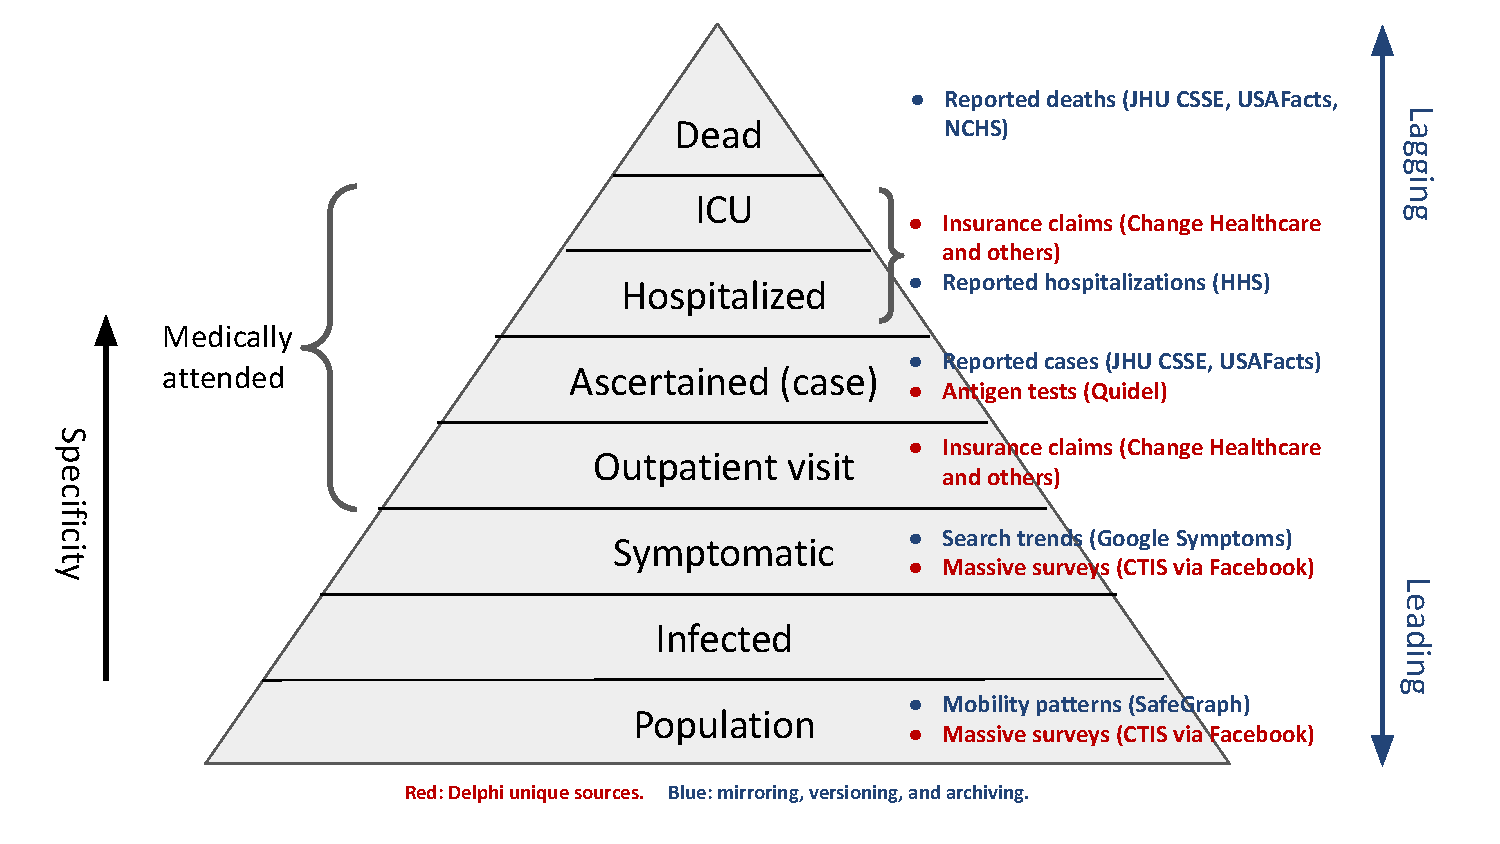
\includegraphics[width=\textwidth]{fig/severity-pyramid.pdf}
\caption{The epidemiological ``severity pyramid'' represents the progression of
cases from the public, through infection, through increasingly severe stages of
disease. The annotations here represent the data sources collected by Delphi's
COVIDcast Epidata API.}
\end{figure}

\clearpage

\begin{figure}

{\centering 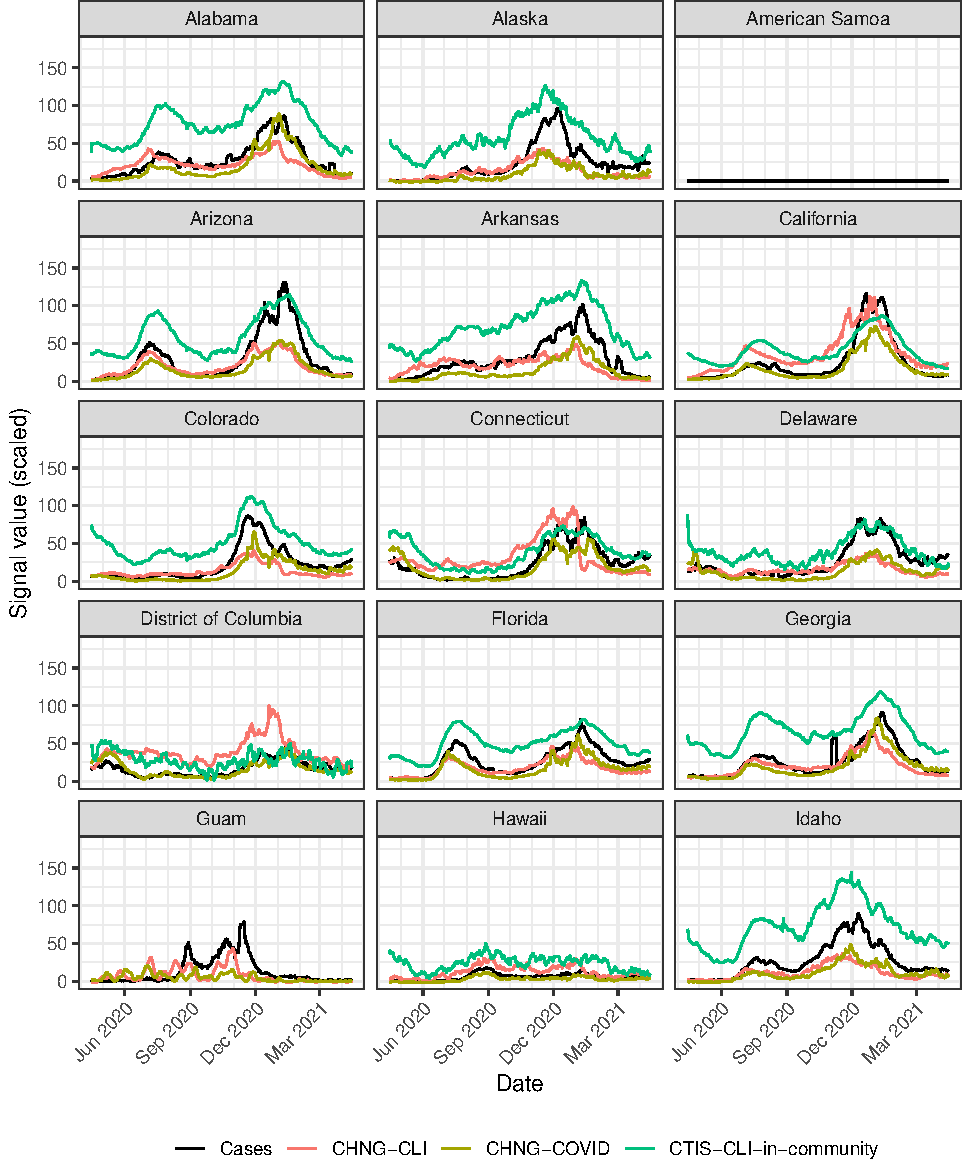
\includegraphics[width=\textwidth]{fig/state-trend-grids-1-1} 

}

\caption{Trends of cases, CHNG-CLI, CHNG-COVID, and CTIS-CLI-in-community for states across the United States. Cases are reported cases per 100,000 population. Other signals are scaled to have the same global maximum across all counties and times, so they can be presented in the same range. (part 1 of 4)}\label{fig:state-trend-grids-1}
\end{figure}

\clearpage

\begin{figure}

{\centering 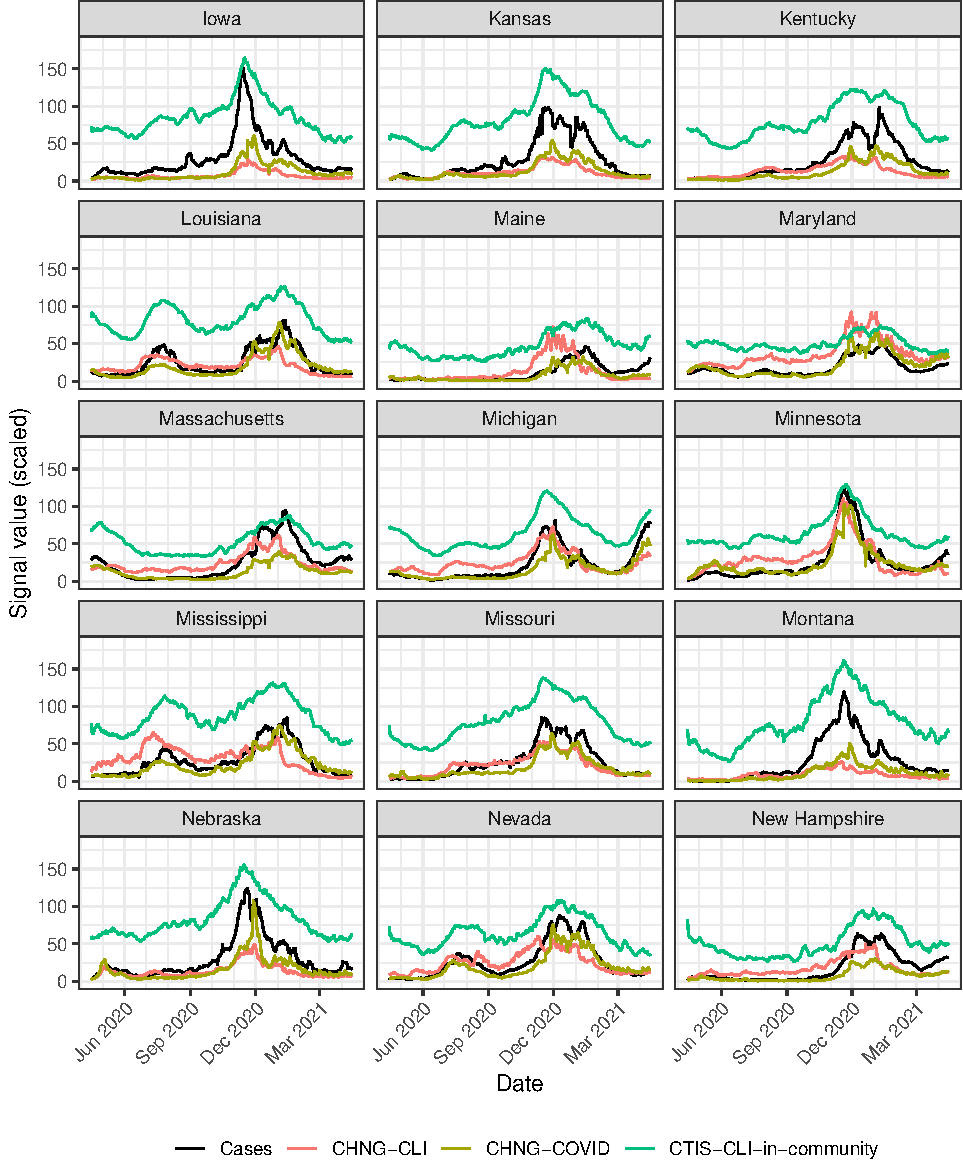
\includegraphics[width=\textwidth]{fig/state-trend-grids-2-1} 

}

\caption{Trends of cases, CHNG-CLI, CHNG-COVID, and CTIS-CLI-in-community for states across the United States. (part 2 of 4)}\label{fig:state-trend-grids-2}
\end{figure}

\clearpage

\begin{figure}

{\centering 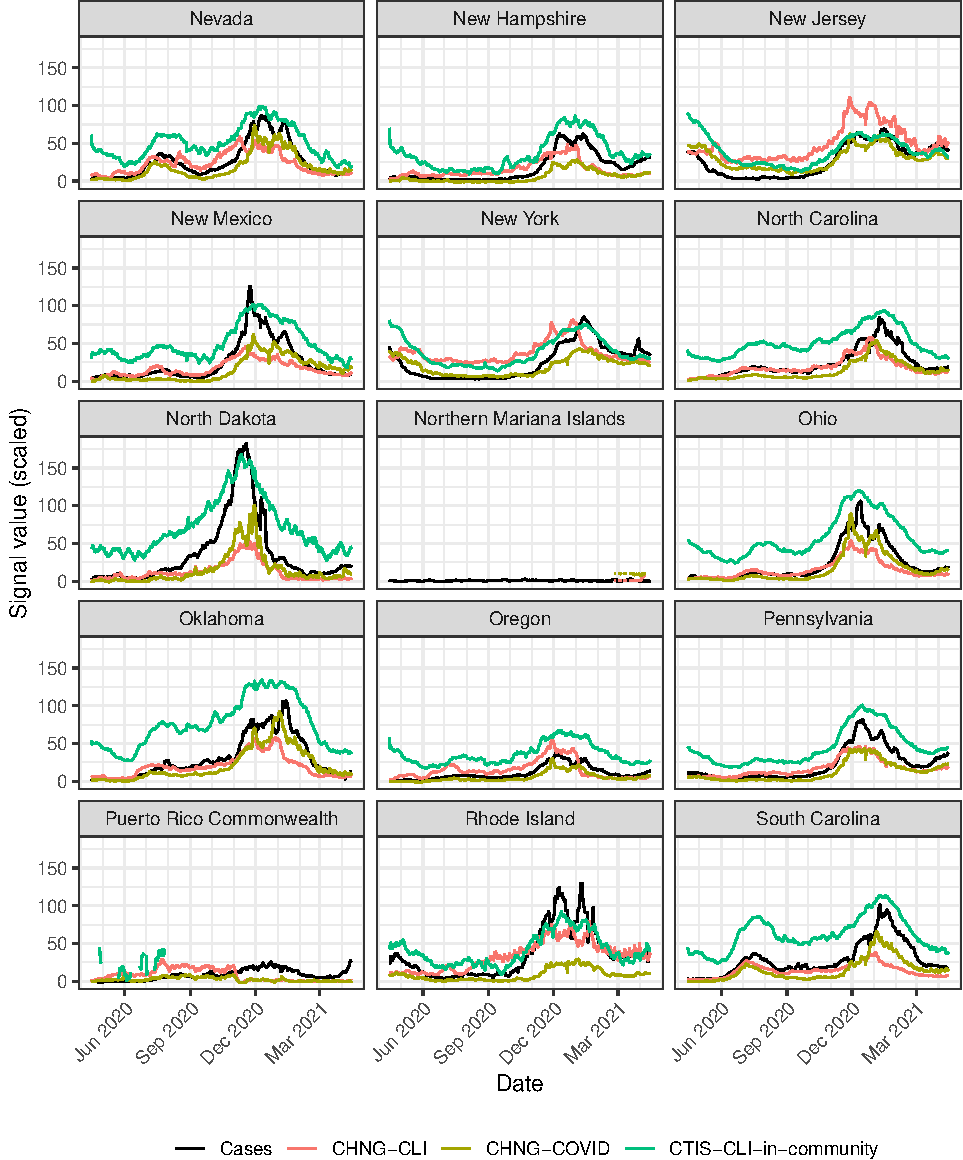
\includegraphics[width=\textwidth]{fig/state-trend-grids-3-1} 

}

\caption{Trends of cases, CHNG-CLI, CHNG-COVID, and CTIS-CLI-in-community for states across the United States. (part 3 of 4)}\label{fig:state-trend-grids-3}
\end{figure}

\clearpage

\begin{figure}

{\centering 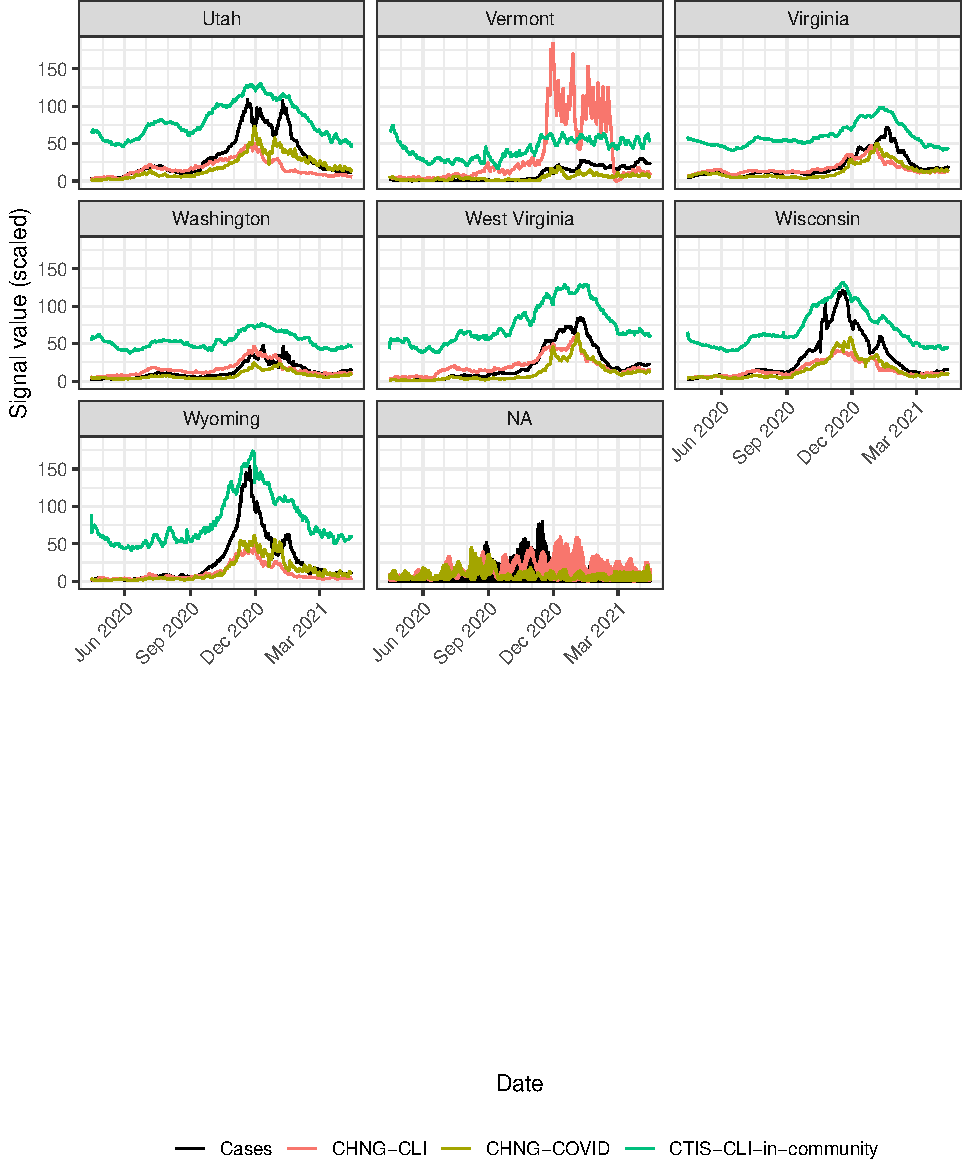
\includegraphics[width=\textwidth]{fig/state-trend-grids-4-1} 

}

\caption{Trends of cases, CHNG-CLI, CHNG-COVID, and CTIS-CLI-in-community for states across the United States. (part 4 of 4)}\label{fig:state-trend-grids-4}
\end{figure}

\clearpage

\begin{figure}

{\centering 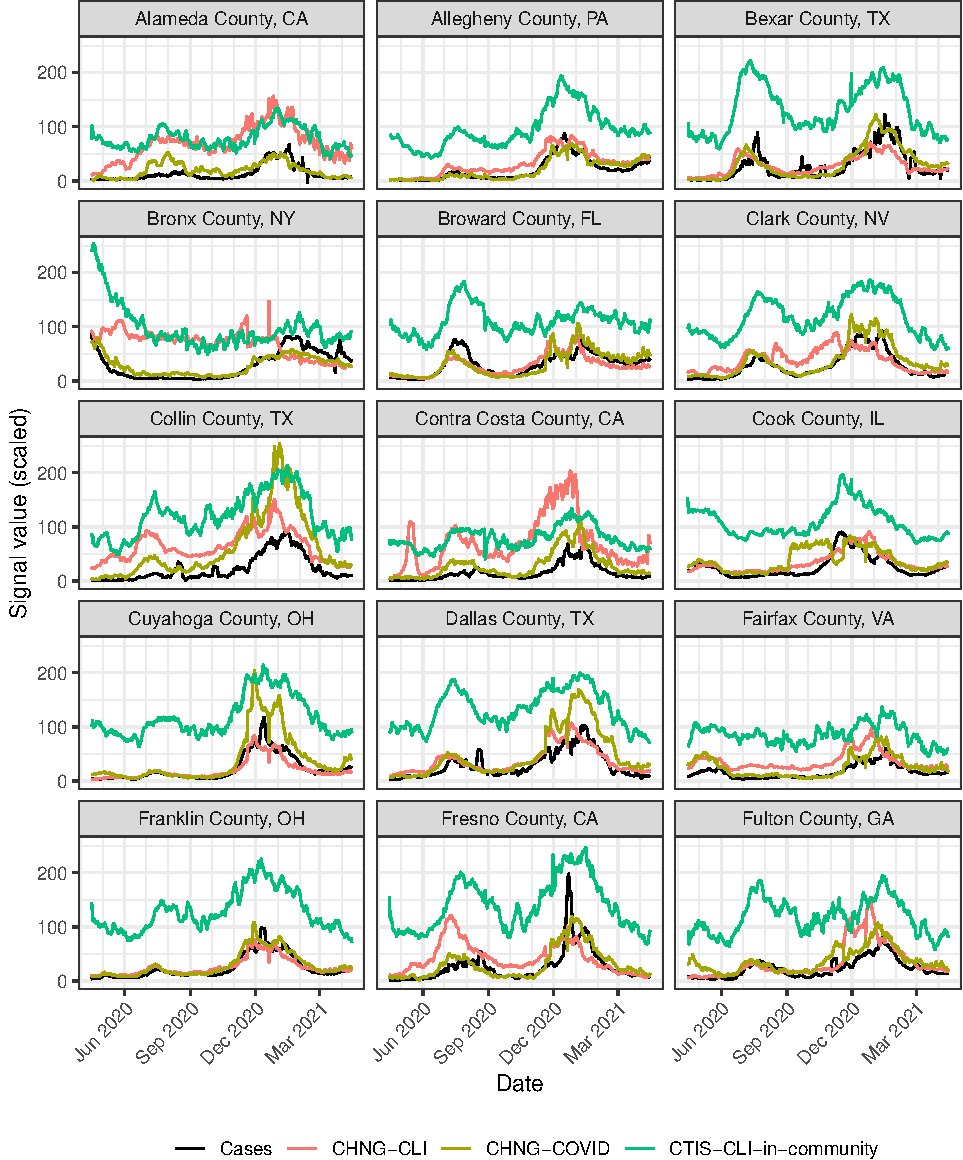
\includegraphics[width=\textwidth]{fig/county-trend-grids-1-1} 

}

\caption{Trends of cases, CHNG-CLI, CHNG-COVID, and CTIS-CLI-in-community for the 50 most populous counties in the United States. Cases are reported cases per 100,000 population. Other signals are scaled to have the same global maximum across all counties and times, so they can be presented in the same range. (part 1 of 4)}\label{fig:county-trend-grids-1}
\end{figure}

\clearpage

\begin{figure}

{\centering 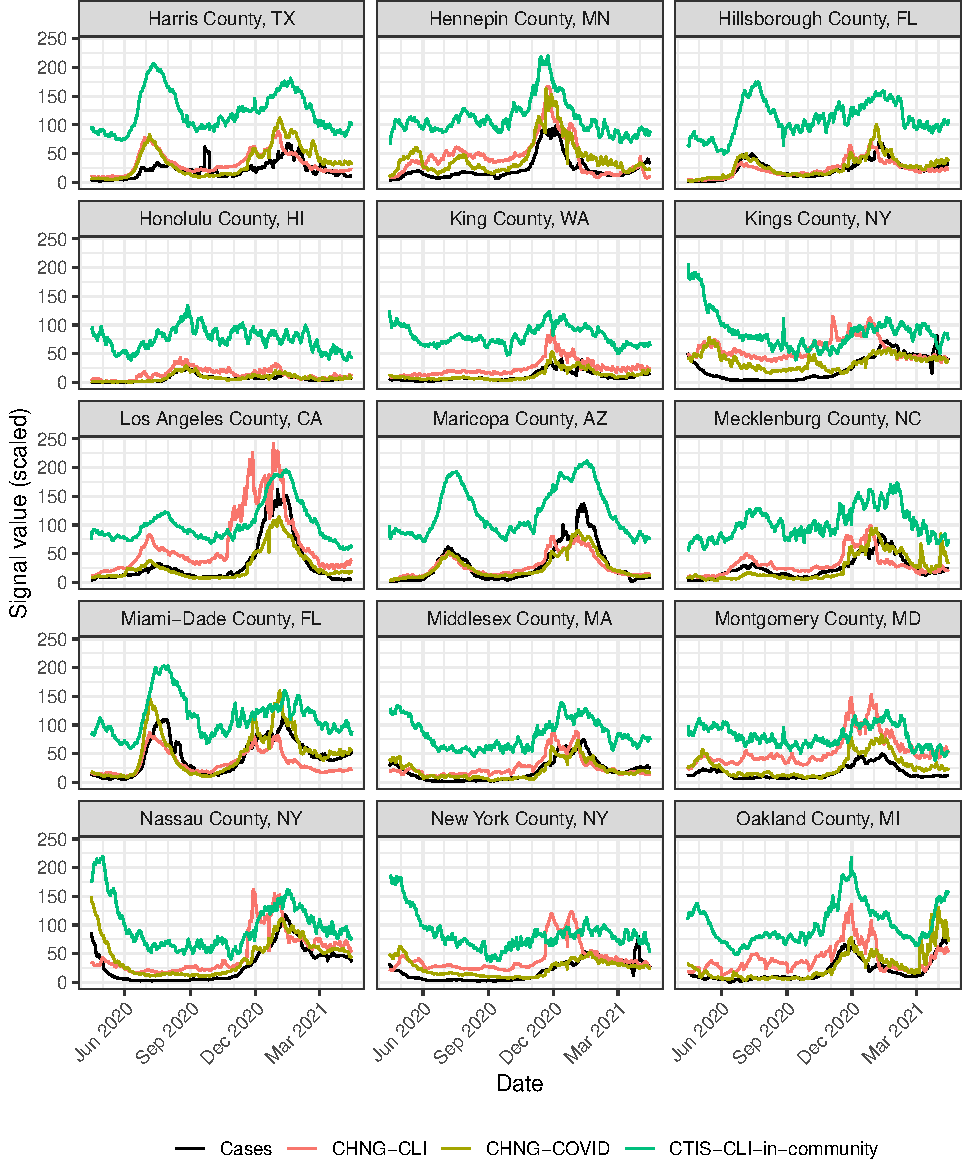
\includegraphics[width=\textwidth]{fig/county-trend-grids-2-1} 

}

\caption{Trends of cases, CHNG-CLI, CHNG-COVID, and CTIS-CLI-in-community for the 50 most populous counties in the United States. (part 2 of 4)}\label{fig:county-trend-grids-2}
\end{figure}

\clearpage

\begin{figure}

{\centering 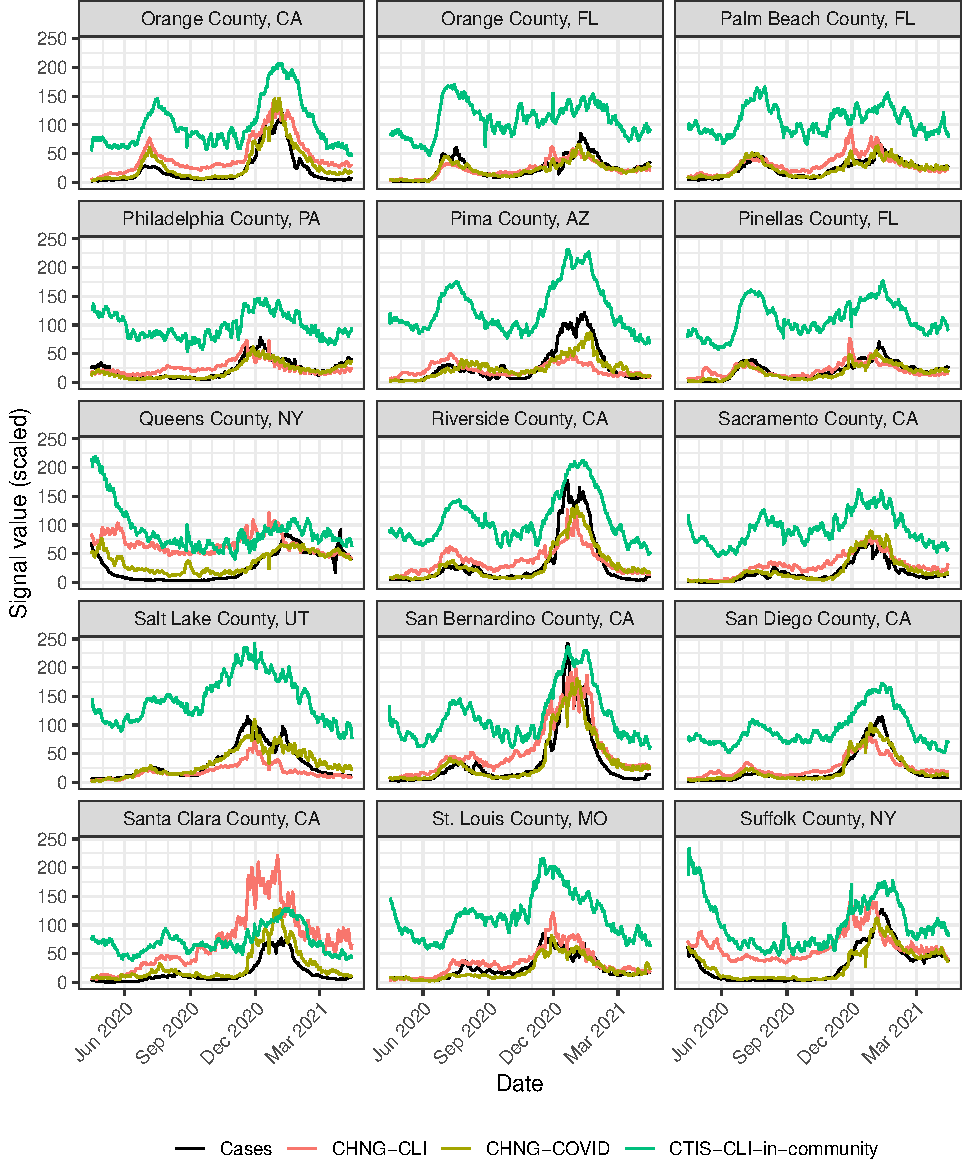
\includegraphics[width=\textwidth]{fig/county-trend-grids-3-1} 

}

\caption{Trends of cases, CHNG-CLI, CHNG-COVID, and CTIS-CLI-in-community for the 50 most populous counties in the United States. (part 3 of 4)}\label{fig:county-trend-grids-3}
\end{figure}

\clearpage

\begin{figure}

{\centering 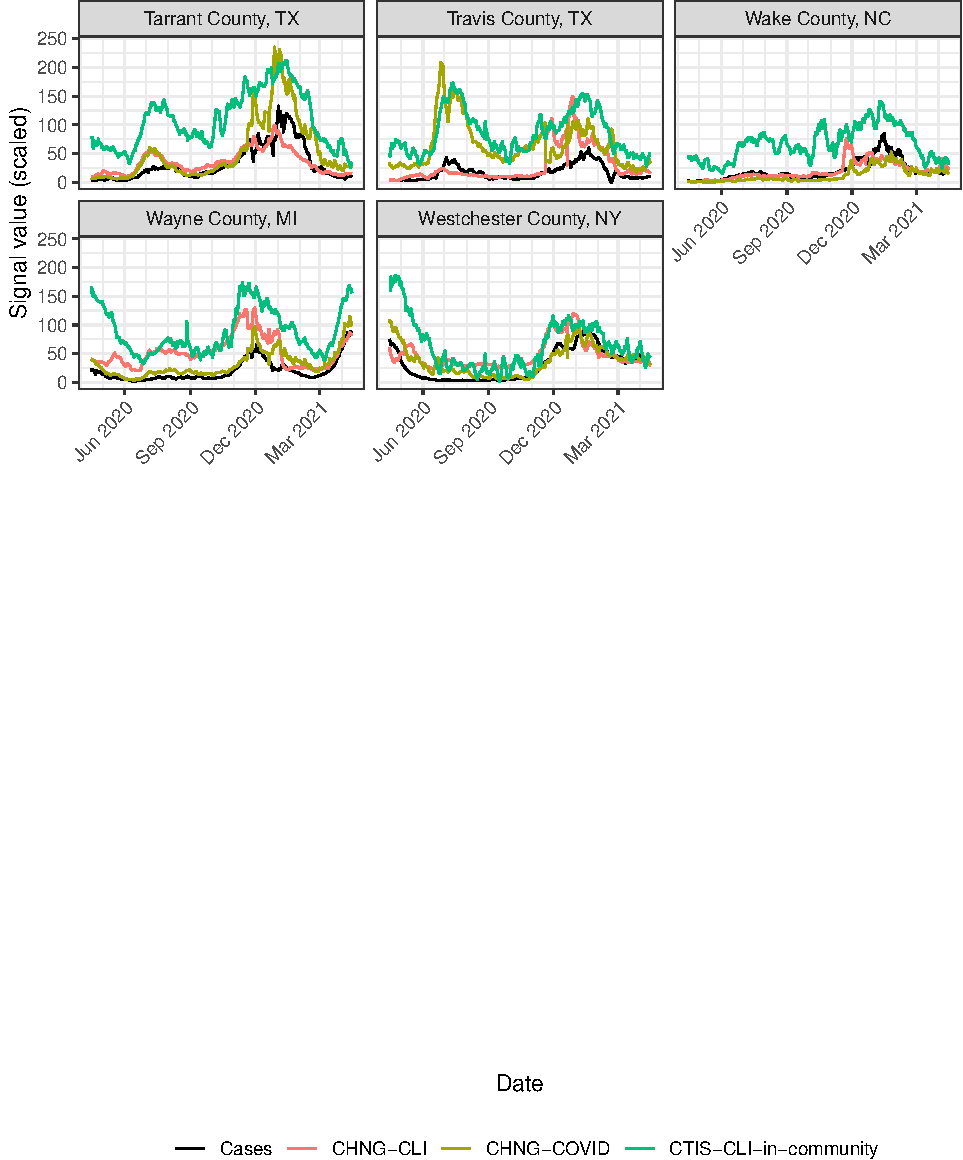
\includegraphics[width=\textwidth]{fig/county-trend-grids-4-1} 

}

\caption{Trends of cases, CHNG-CLI, CHNG-COVID, and CTIS-CLI-in-community for the 50 most populous counties in the United States. (part 4 of 4)}\label{fig:county-trend-grids-4}
\end{figure}

\clearpage

\begin{figure}

{\centering 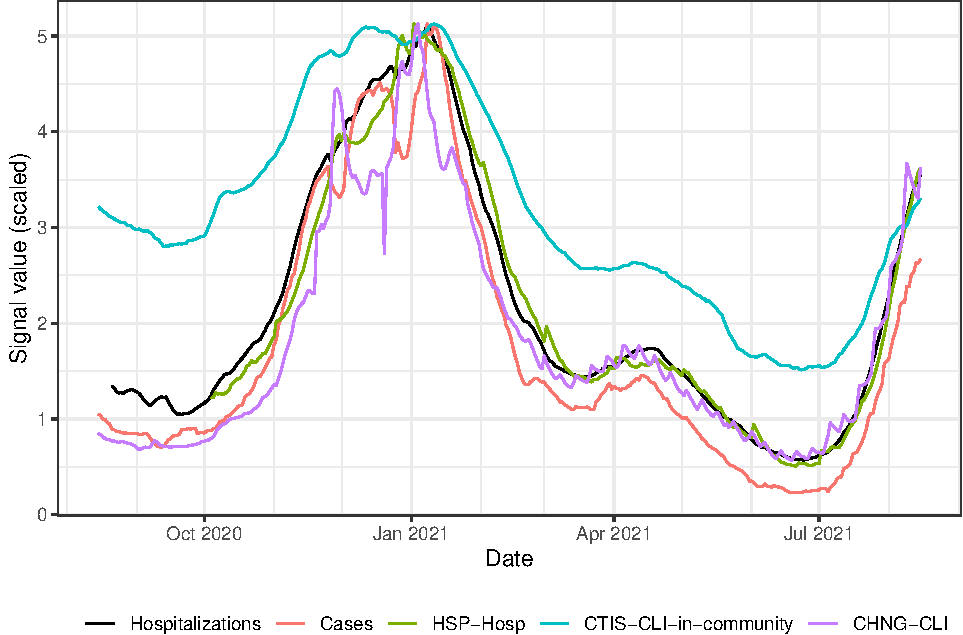
\includegraphics[width=\textwidth]{fig/hospitalization_time_trends_national-1} 

}

\caption{National trends, from August 2020 to August 2021, of HHS-reported confirmed COVID-19 hospital admissions, plus comparison signals in the COVIDcast API. (HHS data was not consistently reported before August 2020.) Here, the HHS data has been processed into a 7-day trailing average rate per 100,000 resident population using Census Bureau estimates for 2019. HSP-Hosp is the percentage of new hospital admissions with COVID-associated diagnoses, based on claims data from health system partners, smoothed in time and adjusted for systematic day-of-week effects (HSP-Hosp is available from an earlier date when working at finer geographical resolutions). HSP-Hosp, CTIS-CLI-in-community, and CHNG-CLI have been scaled to have the same maximum value as the HHS data.}\label{fig:hospitalization_time_trends_national}
\end{figure}

\clearpage

\begin{figure}

{\centering 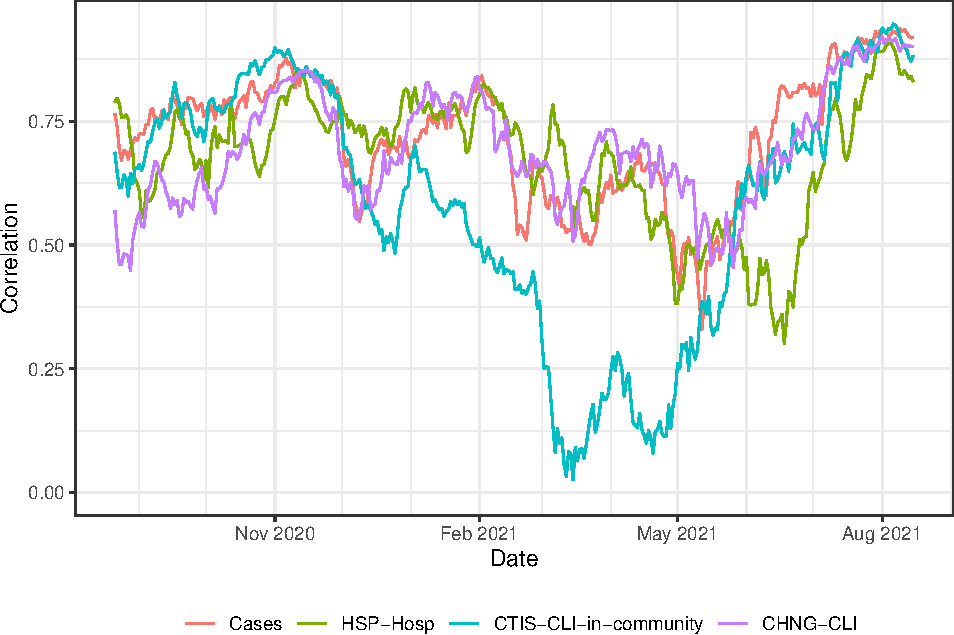
\includegraphics[width=\textwidth]{fig/hosp-correlations-by-time-1} 

}

\caption{Geo-wise correlations with hospitalization rates derived from HHS data, from August 15, 2020 to August 15, 2021, calculated for all times with sufficient available data within this period, over all state-like jurisdictions for which each signal was reported on at least 50 days during this period, limited to state-day combinations for which all signals are available.}\label{fig:hosp-correlations-by-time}
\end{figure}

\begin{figure}

{\centering 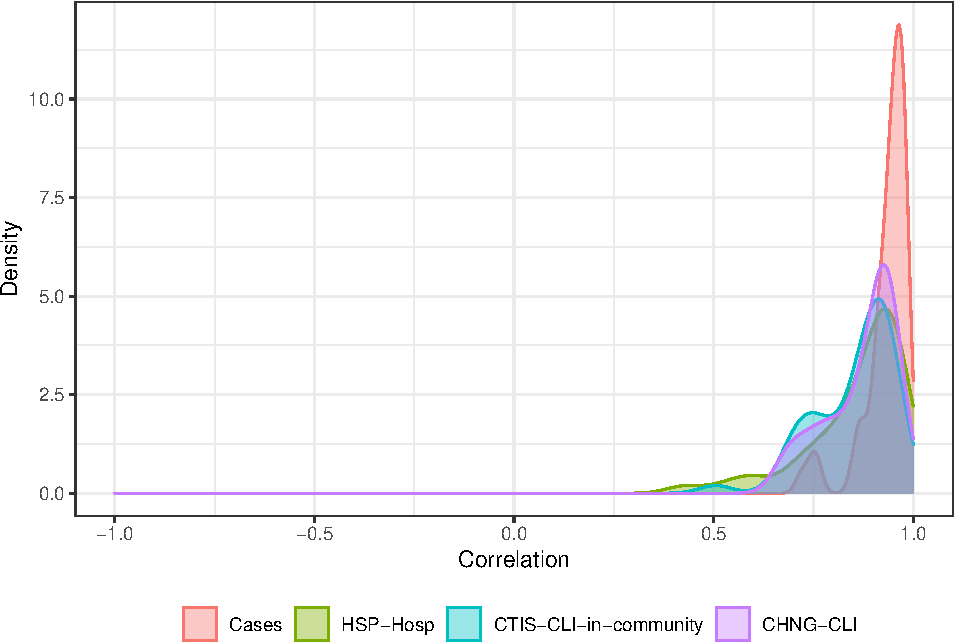
\includegraphics[width=\textwidth]{fig/hosp-correlations-by-state-1} 

}

\caption{Time-wise correlations with hospitalization rates derived from HHS data, from August 15, 2020 to August 15, 2021, calculated over all state-like jurisdictions for which each signal was reported on at least 50 days during this period, limited to state-day combinations for which all signals are available.}\label{fig:hosp-correlations-by-state}
\end{figure}

\FloatBarrier






\bibliography{../../common/covidcast.bib,pnas-materials/pnas-sample.bib}

\end{document}